\documentclass[11pt]{article}
\usepackage{anysize,comment,tcolorbox,multicol,enumitem}
\usepackage{HW}
\usepackage{amsmath}
\usepackage{wrapfig}
\usepackage{enumitem}

\includecomment{comment}
\excludecomment{studentSpace}
%\includecomment{studentSpace}

\includecomment{answer}
\excludecomment{answer}
\includecomment{comment}
\newcommand{\blank}{
\underline{\hspace{1.5cm}\hspace{1.5cm}}
}
\newcommand{\norm}[1]{\left\lVert#1\right\rVert}

\begin{document}
\titleline{\semester}
\exhead{Task 03: Announced 29/01. Due: 10:00 PM,  04-Feb}

\begin{enumerate}

\begin{tcolorbox}
\item  State whether or not the following points are the same and explain why.
\begin{multicols}{2}
\begin{enumerate}[]
\item
$A[2, -1, 3]$, $B[4,-2,6]$
\item
$A[\sqrt{2}/2, -1,0]$, $B[1,-\sqrt{2},0]$
\end{enumerate}
\end{multicols}


\color{blue}
In Projective geometry points $p$ and $p'$ are said to be equivalent $p=kp'$
\begin{enumerate}[]
\item
$A[2, -1, 3]$, $B[4,-2,6]$ Here, we can see that $B = 2A$ so $A$ and $B$ are the same points from the logic explained above.
\item
$A[\sqrt{2}/2, -1,0]$, $B[1,-\sqrt{2},0]$ Similarly, here also, $B=\sqrt{2}A$ so, $A$ and $B$ are same points.
\end{enumerate}

\end{tcolorbox} \begin{tcolorbox}
\item In projective three-space, what are the standard homogeneous
  coordinates of (a) the origin and (b) ideal points determined by the
  intersections of the extensions of the coordinate axes and the ideal
  plane?
  
\color{blue}
\begin{enumerate}[]
\item
Standard homogeneous coordinates of origin in projective three space
: $[0,0,0,1]$ or more generally $[0,0,0,k]$ where $k \in \mathbf{R}$
\item
As we know that intersection of two planes gives a line and intersection of three planes gives a point. And the point given by the intersection of three planes can be found using the cross product. Now the problem of finding the point of intersection between the extension of coordinate axes and the ideal plane can be re-framed as finding the intersection between three planes as we know intersection of two planes will give us a point.\\
Ideal Plane: $[0,0,0,1]$, zx-plane: $[0,1,0,0]$, xy-plane: $[0,0,1,0]$ and yz-plane: $[1,0,0,0]$. Now the Intersection of xy-plane and xz-plane will give the x-coordinate line and similarly, xz-plane and yz-plane will give z-coordinate line and xy-plane and yz-plane will give y-coordinate line. With this knowledge we find the intersection point of the extension of the x-axis and ideal plane will be:

\begin{equation*}
    \begin{vmatrix}
        p_1 & p_2 & p_3 & p_4\\ 
        0 & 0& 0& 1\\
        0& 0& 1& 0\\
        0& 1& 0& 0
        \end{vmatrix} = [-1, 0, 0, 0]
\end{equation*}
Similarly, the intersection point of the extension of the y-axis and ideal plane will be:
\begin{equation*}
    \begin{vmatrix}
        p_1 & p_2 & p_3 & p_4\\ 
        0 & 0& 0& 1\\
        0& 0& 1& 0\\
        1& 0& 0& 0
        \end{vmatrix} = [0, -1, 0, 0]
\end{equation*}

and the intersection point of the extension of the y-axis and ideal plane will be:
\begin{equation*}
    \begin{vmatrix}
        p_1 & p_2 & p_3 & p_4\\ 
        0 & 0& 0& 1\\
        0& 1& 0& 0\\
        1& 0& 0& 0
        \end{vmatrix} = [0, 0, -1, 0]
\end{equation*}


\end{enumerate}

\end{tcolorbox} \begin{tcolorbox}
\item Write standard homogeneous coordinates for the points specified
  in uppercase characters. (Use left and right to distinguish.)
\begin{multicols}{2}
\centering
\vspace*{55px}
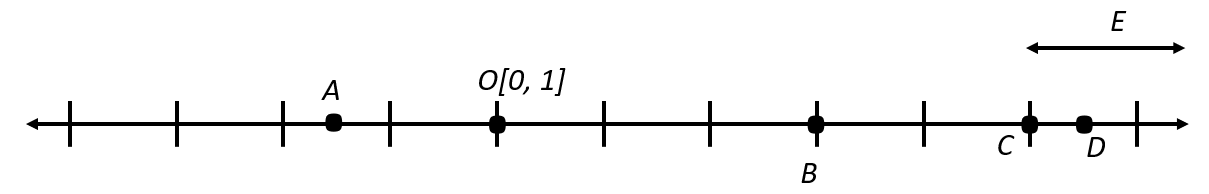
\includegraphics[width=0.9\linewidth]{images/Q3a.PNG}
\label{fig:q3a}
\vfill\null
\columnbreak
\centering
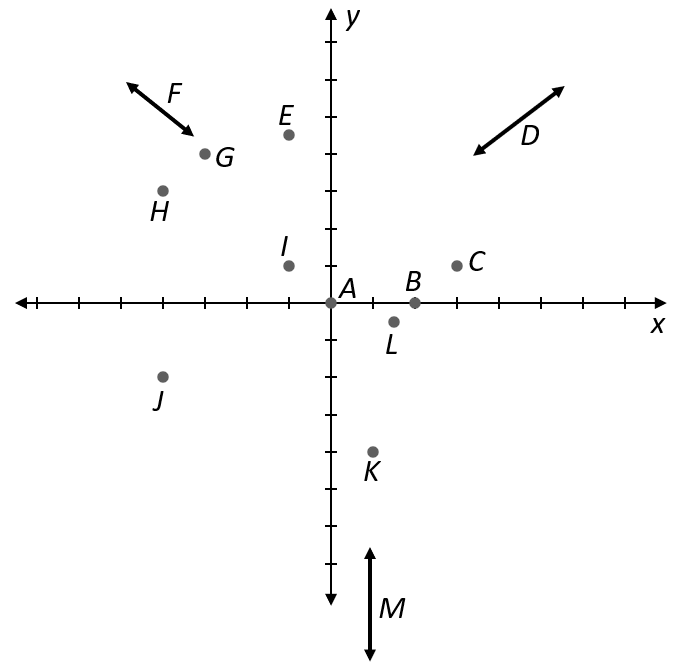
\includegraphics[width=0.9\linewidth]{images/Q3b.PNG}
\label{fig:q3b}
\end{multicols}

\color{blue}
Assuming left side is the projective one space and second to be projective two space.
\begin{enumerate}[]
\item[Left: ]
$A: [-1.5,1]$, 
$B: [3,1]$, 
$C: [5,1]$, 
$D: [5.5,1]$, 
$E: [5.5,0]$.

\item[Right:] 
$A: [0,0,1]$, 
$B: [2,0,1]$, 
$C: [3,1,1]$,
$D: [4.5,5,0]$, 
$E: [-1,4.5,1]$, 
$F: [-4,5,0]$, 
$G: [-3,4,1]$, 
$H: [-4,3,1]$, 
$I: [-1,1,1]$,
$J: [-4,-2,1]$,
$K: [1,-4,1]$,
$L: [1.5,-0.5,1]$,
$M: [1,0,0]$.


\end{enumerate}

\end{tcolorbox} \begin{tcolorbox}
\item Which of the following points lie on the line $3p_1 -2p_2+5p_3 =
  0$?  Why?
\begin{multicols}{2}
\begin{enumerate}[]
\item
$A[1,1,2]$
\item
$B[4,1,-2]$
\end{enumerate}
\end{multicols}
\begin{enumerate}[]
\color{blue}
\item
{ For a point to be on a line $line^T point = 0$. But, $3*1-2*1+5*2 \neq 0$ Hence, point $A[1,1,2]$ does not lie on the line $3p_1 -2p_2+5p_3 =
  0$.
  \item
  Similarly, $3*4-2*1-5*2 = 0$. Hence, the point $B[4,1,-2]$ lies on the line $3p_1 -2p_2+5p_3 =
  0$}
  \end{enumerate}

\end{tcolorbox} \begin{tcolorbox}
\item Write the coordinates of the lines that are the extensions to the
  projective plane of the following Euclidean lines.
\begin{multicols}{2}
\begin{enumerate}[]
\item
$3x + 2y = 6$
\item
$4x + 5y + 7 = 0$
\end{enumerate}
\end{multicols}
\color{blue}
If $l$ and $\mathbf{x}$ are a line and a point in projective two space, and the point lies on the line then:
\begin{equation*}
    l^T \mathbf{x} = 0
\end{equation*}
\begin{enumerate}[]
\item
So, the line $3x + 2y = 6$ can be written as $3x + 2y -6 = 0$. Hence the lines in projective space become:  $l = [3,2,-6]$.
\item
Similarly, line $4x + 5y + 7 = 0$ in projective space becomes: $l = [4,5,7]$.
\end{enumerate}

\end{tcolorbox} \begin{tcolorbox}
\item Sketch each line in the projective plane whose equation is given.
\begin{multicols}{2}
\begin{enumerate}[]
\item
$2p_1 + 3p_2 + 5p_3 = 0$
\item
$3p_1 - 2p_2 - p_3 = 0$
\end{enumerate}
\end{multicols}
\color{blue}
Let Line defined in (a) $2p_1 + 3p_2 + 5p_3 = 0$ be Line-A (Blue line) and line defined in (b) by $3p_1 - 2p_2 - p_3 = 0$ be Line-B (Green line). The sketch of both line is given in the figure-  below:\\

\centering
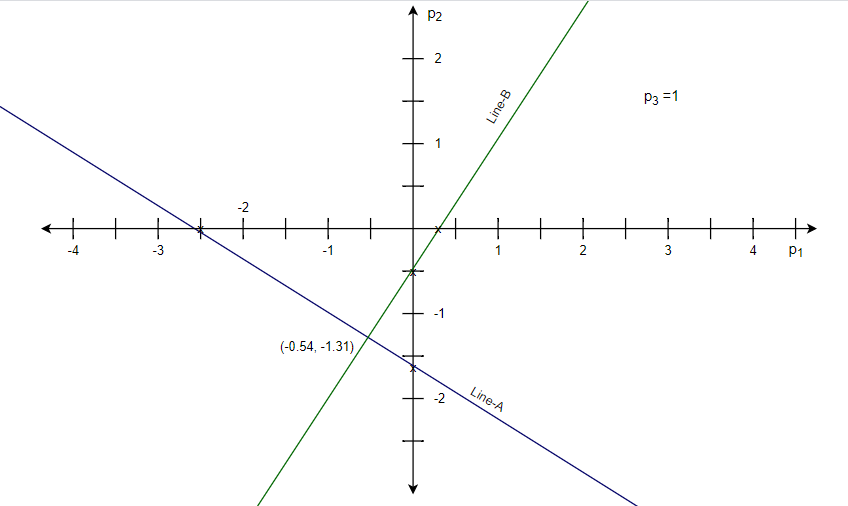
\includegraphics[width=0.95\linewidth]{images/Q6.PNG}
\label{fig:q6}

\end{tcolorbox} \begin{tcolorbox}
\item  In each of the following cases, sketch the line determined by the two given points; then find the equation of the line.
\begin{multicols}{2}
\begin{enumerate}[]
\item
$A[3, 1, 2]$, $B[1,2,-1]$
\item
$A[2,1,3]$, $B[1,2,0]$
\end{enumerate}
\end{multicols}
\color{blue}
Let points defined in (a) $A[3, 1, 2]$ and $B[1,2,-1]$ be $A_1$ and $B_1$ and points defined in (b) $A[2,1,3]$, $B[1,2,0]$ be $A_2$ and $B_2$. Line-A is the lines joining the points $A_1$ and $B_1$ and Line-B is the lines joining the points $A_2$ and $B_2$. The sketch of both lines and points is given in the figure-  below:\\

\begin{center}
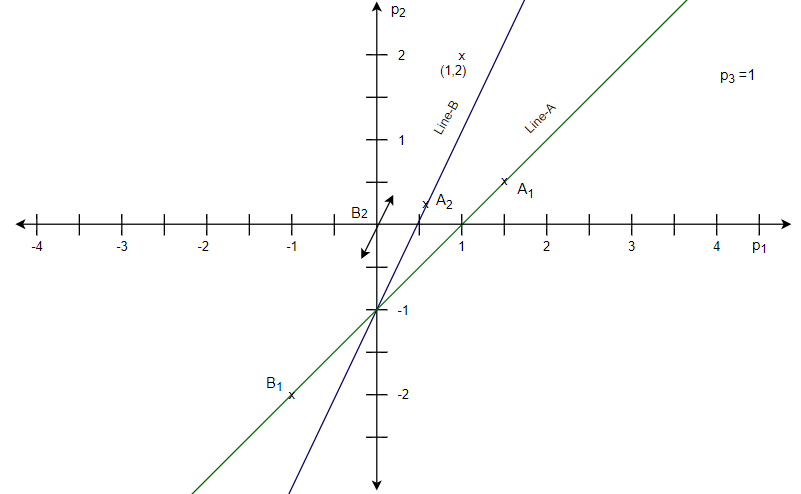
\includegraphics[width=\linewidth]{images/Q7.PNG}
\label{fig:q7}
\end{center}

Equation of lines can be found using cross product as
\begin{enumerate}[]
\item
\begin{gather*}
    \begin{vmatrix}
        p_1 & p_2 & p_3 & \\ 
        3 & 1 & 2\\
        1 & 2 & -1\\
    \end{vmatrix} = -5p_1+5p_2+5p_3 = 0.
    \\
    \text{Line-A} \Rightarrow -5p_1+5p_2+5p_3 = 0, or -p_1+p_2+p_3 = 0 
\end{gather*}

\item
\begin{gather*}
    \begin{vmatrix}
        p_1 & p_2 & p_3 & \\ 
        2 & 1 & 3\\
        1 & 2 & 0\\
    \end{vmatrix} = -6p_1+3p_2+3p_3 = 0.
    \\
    \text{Line-B} \Rightarrow -6p_1+3p_2-p_3 = 0, or -2p_1+p_2+p_3 = 0 
\end{gather*}
\end{enumerate}

\end{tcolorbox} \begin{tcolorbox}
\item  Find the standard homogeneous coordinates of the point of
  intersection for each pair of lines. 
\begin{multicols}{2}
\begin{enumerate}[]
\item
$p_1 + p_2 - 2p_3 = 0, 3p_1 + p_2 + 4p_3 = 0$
\item
$p_1 + p_2 = 0, 4p_1 - 2p_2 + p_3 = 0$
\end{enumerate}
\end{multicols}

\begin{enumerate}[]
\color{blue}
\item
{ Point of intersection of a line in homogeneous coordinate is cross product between the line.\\
\begin{equation*}
=
    \begin{vmatrix}
        i & j & k & \\ 
        1 & 1 & -2\\
        3 & 1 & 4\\
    \end{vmatrix} = 6i-10j-k. 
\end{equation*}
Hence, the point of intersection is $[6,-10,-2]$
}
  \item
  Similarly, point of intersection for lines $p_1 + p_2 = 0, 4p_1 - 2p_2 + p_3 = 0$
\begin{equation*}
=
    \begin{vmatrix}
        i & j & k & \\ 
        1 & 1 & 0\\
        4 & -2 & 1\\
    \end{vmatrix} = i-j-6k. 
\end{equation*}
Hence, the point of intersection is $[1,-1,-6]$
  \end{enumerate}

\end{tcolorbox} \begin{tcolorbox}
\item  Determine which of the following sets of three points are collinear. 
\begin{multicols}{2}
\begin{enumerate}[]
\item
$A[1,2,1]$, $B[0,1,3]$, $[2,1,1]$
\item
$A[1,2,3]$, $B[2,4,3]$, $[1,2,-2]$
\end{enumerate}
\end{multicols}
\begin{enumerate}[]
\color{blue}
\item
{ For Points to be collinear, the determinant of $[A^T B^T C^T]$ should be zero\\
\begin{equation*}
    \Rightarrow
    \begin{vmatrix}
        1 & 0 &  2 \\ 
        2 & 1 & 1\\
        1 & 3 & 1\\
    \end{vmatrix} = -2+ 5 \neq 0. 
\end{equation*}
Hence, the points $A[1,2,1]$, $B[0,1,3]$, $[2,1,1]$ are not collinear.
}
  \item
  Similarly,
\begin{equation*}
     \Rightarrow
    \begin{vmatrix}
        1 & 2 & 1 \\ 
        2 & 4 & 2\\
        3 & 3 &-2\\
    \end{vmatrix} = -14 + 20 - 6 = 0. 
\end{equation*}
Hence, the points $A[1,2,3]$, $B[2,4,3]$, $[1,2,-2]$ are collinear.
Hence, the point of intersection is $[1,-1,-6]$
\end{enumerate}

\end{tcolorbox} \begin{tcolorbox}
\item  Determine which of the following sets of three lines meet in a
  point. 
\begin{multicols}{2}
\begin{enumerate}[]
\item
$l[1,0,1], m[1,1,0], n[0,1,-1]$
\item
$l[1,0,-1], m[1,-2,1], n[3,-2,-1]$
\end{enumerate}
\end{multicols}

\begin{enumerate}[]
\color{blue}
\item
{ For checking if three line meet in a point we can check for the point of intersection of two different permutations of line and if they meet in same point then we can say they meet at the same point.\\
Checking for line $l$ and $m$:
\begin{equation*}
\begin{vmatrix}
        i & j &  k \\ 
        1 & 0 & 1\\
        1 & 1 & 0\\
    \end{vmatrix} \Rightarrow [-1, 1, 1]. 
\end{equation*}
Checking for line $m$ and $n$:
\begin{equation*}
\begin{vmatrix}
        i & j &  k \\ 
        1 & 1 & 0\\
        0 & 1 & -1 \\
    \end{vmatrix} \Rightarrow [-1, 1, 1]. 
\end{equation*}
Line $l$ and $m$ meet at the same point as line $m$ and $n$ hence, line $l$, $m$, $n$ meet in a point.
}
  \item
  Similarly,
Checking for line $l$ and $m$:
\begin{equation*}
\begin{vmatrix}
        i & j &  k \\ 
        1 & 0 & -1\\
        1 & -2 & 1\\
    \end{vmatrix} \Rightarrow [-2, -2, -2]. 
\end{equation*}
Checking for line $l$ and $n$:
\begin{equation*}
\begin{vmatrix}
        i & j &  k \\ 
        1 & 0 & -1 \\
        3 & -2 & -1 \\
    \end{vmatrix} \Rightarrow [-2, -2, -2]. 
\end{equation*}
Line $l$ and $m$ meet at the same point as line $m$ and $n$ hence, line $l$, $m$, $n$ meet in a point.
\end{enumerate}
\end{tcolorbox}

\end{enumerate}


\end{document}

